\documentclass[a4paper,norsk]{article}
\usepackage{preamble}
\usepackage{tabu}
\usepackage{color, colortbl}
\definecolor{LightCyan}{rgb}{0.88,1,1}
\usepackage{graphicx}
\usepackage{caption}
\usepackage{subcaption}

\begin{document}

\section*{TASK 2: Discretization of convection/diffusion}
\textbf{Derive a proper variational formulation of the convection/diffusion 
problem.  Derive sucient conditions that make the problem well-posed.  Discuss
why oscillations appear for standard Galerkin methods and show how SUPG
methods resolve these problems.  Discuss also approximation properties in
light of Cea's lemma.}\newline \newline

The convection–diffusion equation is a combination of the diffusion and convection (advection) equations, and describes physical phenomena where particles, energy, or other physical quantities are transferred inside a physical system due to two processes
\begin{align*}
\mu \nabla^2 u +v \cdot \nabla u = f \hspace{1mm} \in \Omega \\
u = g \hspace{1mm} \in \partial \Omega
\end{align*}

\begin{itemize}
\item u = Is the 
\item $\mu \nabla^2 u$ = Diffusion term, distribution of consentration due to consentration differene (Ink in glass..)
\item $\mu$ = Dynamic viscoucity
\item $v \cdot \nabla u $ = Convection(Advection), distribution of consentration due to fluid flow
\item v = Can bee fluid flow average, etc..
\end{itemize}

\subsection*{Singular Pertubation problem}
Consequence $\mu \rightarrow 0$, boundary conditions can't be satisfied. Changes the very nature of problem.
Practical situations $\mu > 0$, but small in the sence that $\mu << |v|$. This results in a overdetermined problem. (Also if $\mu$ goes to 0).
For such problem where $\mu << |v|$, solution will be similar to  $\mu = 0$, EXCEPT close to \textbf{NON-inflow boundary}. Here we will typically have a boundary layer.
We will also observe that the discretized problem, will result in unphysical oscillations starting at this boundary layer.

\newpage
\subsection{1D con-diff problem}
\begin{align*}
\ u_x - \mu u_{xx}  = 0 \\
u(0) = 0 \hspace{2mm} u(1) = 1 \\
u_e(x) = \frac{e^{\frac{-x}{\mu}} -1}{e^{\frac{-1}{\mu}} - 1}
\end{align*}

For $\mu \rightarrow 0$ both $e^{\frac{-x}{\mu}}$ and $e^{\frac{-1}{\mu}}$ and $u(x) \approx 1$ unless $x \approx 0$. Close to the inflow boundary
x = 0, there will be a boundary layer where u has exponential growth.
\newline \textbf{Galerkin method} \newline

Find $u \in  H^1_{0,1}$ such that 
\begin{align*}
\int_0^1 \big( u_x v - \mu u_{xx} v \big) \hspace{1mm} dx = 0 \\
\inner[-u_x]{v} \hspace{2mm} \mu \inner[\nabla u]{\nabla v} = 0 \hspace{2mm}  \forall v \in H^1_{0,0}
\end{align*}

\begin{figure}[h!]
	\centering
	\caption*{CONVEC N = 20 and N = 100}
	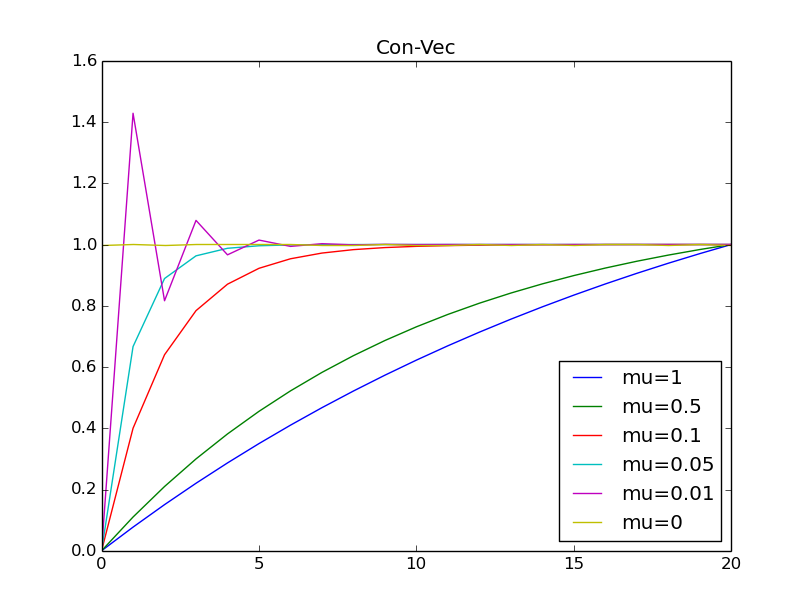
\includegraphics[scale=0.32]{convec.png}
	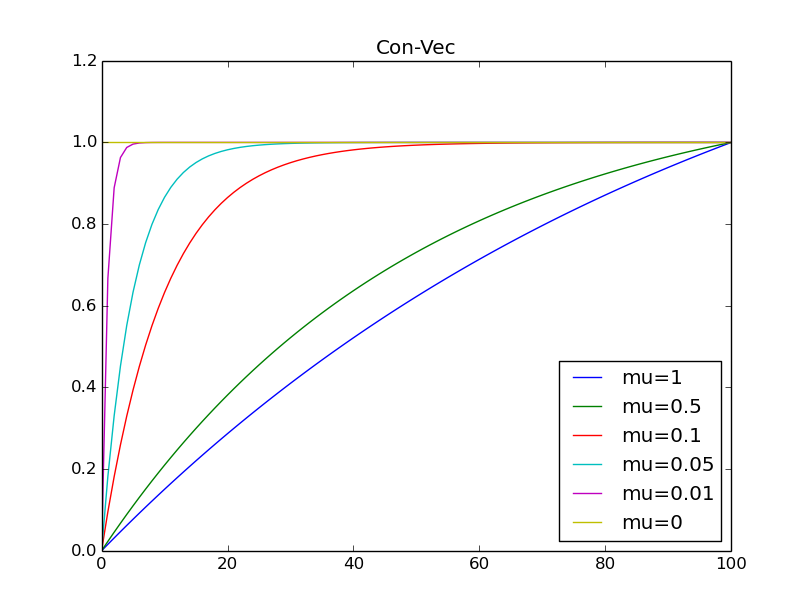
\includegraphics[scale=0.32]{convechighn.png}
\end{figure}
Observe oscillations for low choice of N. WHY DO THIS HAPPEND? Explain with FDM.
Using central difference
\begin{align*}
&\frac{\mu}{h^2}\Big[u_{i+1} - 2u_{i} + u_{i-1} \Big] - \frac{v}{2 h} \Big[u_{i+1} - u_{i-1} \Big] = 0 \\
&u_0 = 0 \hspace{2mm} u_N = 1 \hspace{3mm} \\ 
\text{for} \hspace{2mm} \mu = 0 \\
&\frac{v}{2 h} \Big[u_{i+1} - u_{i-1} \Big] = 0 \hspace{3mm} u_{i+1} = u_{i-1} \hspace{2mm} \textbf{SOURCE OSCILLATIONS}
\end{align*}
\newpage
\textbf{THE CURE} Introduce and artifical diffusion term. \\ drop central difference scheme, use upwind such that 
\begin{align*}
\pd[u]{x} (x_i) = \frac{u_{i+1}-u_{i}}{h} \hspace{2mm} v < 0 \\
\pd[u]{x} = \frac{u_{i}-u_{i-1}}{h} \hspace{2mm} v > 0
\end{align*}
\begin{itemize}
\item \textbf{PROS} = Oscillations dissapear
\item \textbf{CONS} = 1 order convergence
\end{itemize}
\textbf{POINT!} Show relation to \textbf{upwind} and \textbf{artifical diffusion}
Observe 
\begin{align*}
&\frac{u_{i+1}-u_{i-1}}{2h} \hspace{2mm} \textbf{Central Scheme, 1. order convergence} \\
&+ \frac{h}{2} \frac{-u_{i+1} + 2u_{i} - u_{i-1}}{h^2} \hspace{2mm} \textbf{Central Scheme, 2.order derivative} \\
&= \frac{u_i - u_{i-1}}{h} \hspace{2mm} \textbf{Upwind scheme} \\
&\text{Add diffusion as} \hspace{2mm} \epsilon = \frac{h}{2} \\
&-u_x - (\mu + \epsilon) u_{xx} = 0
\end{align*}
Hard to derive in FEM, but in same sence adding som kind of diffution term such that 
\begin{align*}
-u_x - (\mu + \beta h) u_{xx} = 0 \hspace{3mm} \beta = 0.5,  h = \text{mesh.hmin()}
\end{align*}
Changes our variational problem to
Find $u \in  H^1_{0,1}$ such that 
\begin{align*}
\inner[-u_x]{v} \hspace{2mm} (\mu + \beta h) \inner[\nabla u]{\nabla v} = 0 \hspace{2mm}  \forall v \in H^1_{0,0}
\end{align*} 


\begin{figure}[h!]
	\centering
	\caption*{CONVEC N = 20 and N = 100}
	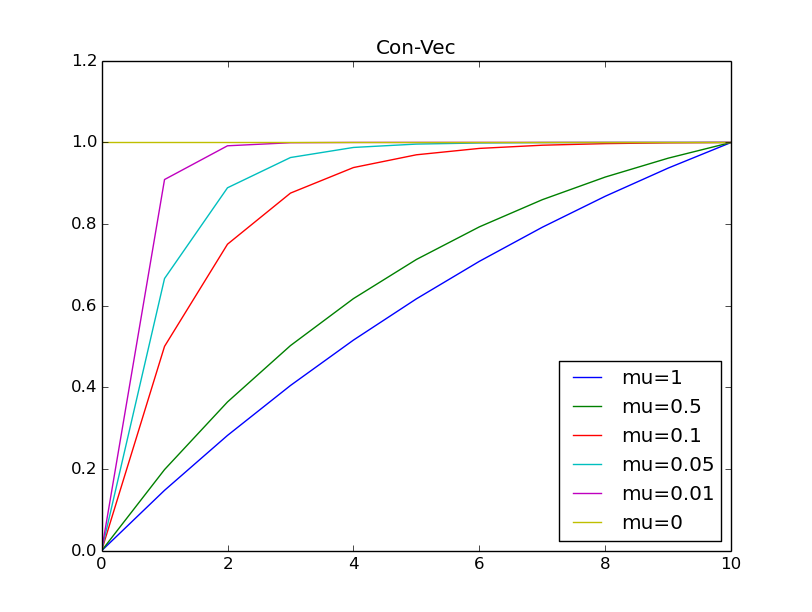
\includegraphics[scale=0.34]{convecart.png}
	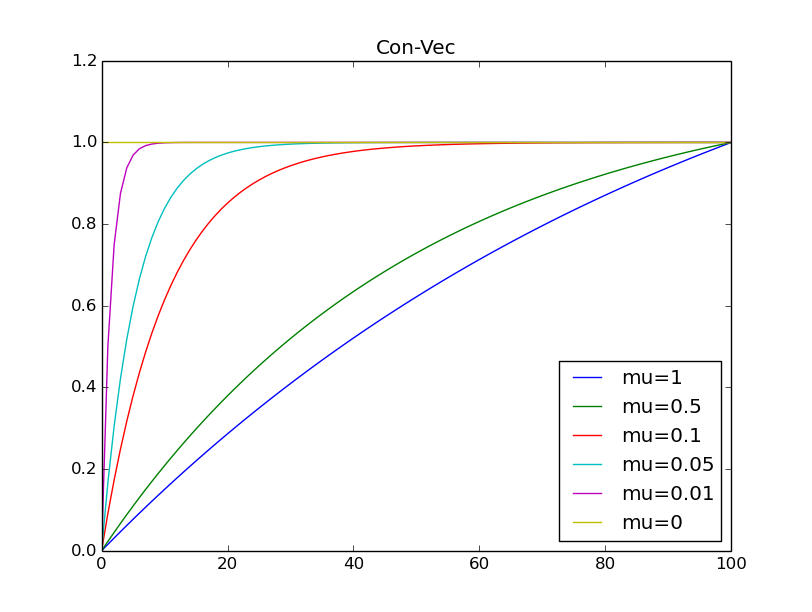
\includegraphics[scale=0.34]{convecarthighn.png}
\end{figure}
\newpage

\subsection*{Petrov-Galerkin Method}
Why bother ? Isn't artifical diffution good enough ?? \newline
Find $u \in  H^1_{0,1}$ such that 
\begin{align*}
\int_0^1 \big( u_x v - \mu u_{xx} v \big) \hspace{1mm} dx = 0 \\
\inner[-u_x]{v} + \hspace{2mm} \mu \inner[\nabla u]{\nabla v} = 0 \hspace{2mm}  \forall v \in H^1_{0,0} \\
a(u, v)  = b(v)  \hspace{2mm}  \forall v \in H^1_{0,0} \\
\end{align*}

\begin{align*}
&a(u, v) = \int_{\Omega} \big( \mu \inner[\nabla u]{\nabla v} + v \cdot \nabla u \big) \hspace{1mm} dx \\
&b(v) = \int_\Omega f v \hspace{1mm} dx
\end{align*}
IT IS A QUESTION OF CONSITICY!! \newline
Standard Galerkin
Find $u_h \in V_{h, g}$
\begin{align*}
a(u_h, v_h) = (f, v_h) \hspace{2mm} \forall v_h \in V_{h, 0}
\end{align*}
After introducing ARTDIFF
\begin{align*}
a(u_h, v_h) + \frac{h}{2} (\nabla u_h, \nabla v_h) = (f, v_h) \hspace{2mm} \forall v_h \in V_{h, 0}
\end{align*}
Introducing truncation error $\tau$ as 
\begin{align*}
\tau(u_h, v_h) = a(u_h, v_h) - (f, v_h) 
\end{align*} 
Standard Galerkin is \textbf{STRONGLY CONSISTANT} by Galerkin-orthogonality, such that $\tau(u) = 0$ for every discretization \newline
Artificial diffusion is \textbf{CONSISTANT} in the way that 
\begin{align*}
\tau(u) = \sup_{v \in V_h} \frac{\tau(u, v_h)}{||v||_H} \approx \mathcal{O}(h) \\
\lim_{h \to 0} \tau(u) \rightarrow 0
\tau(u_h, v_h) = a(u_h, v_h) - (f, v_h) = a(u_h - h, v_h) = 0 
\end{align*}
It will approach zeros as $h \rightarrow 0$ only.
Therefore we will introduce Petrov-Galerkin, a strongly consistent diffusion by em-
ploying alternative test functions. Using a clever alternative test function
\begin{align*}
a(u_h, w_h) = (f, w_h) \hspace{2mm} \forall w_h \in V_{h, 0}
\end{align*}

\newpage
\section*{TASK 5: Iterative methods}
\textbf{Describe the Richardson iteration.  Explain spectral equivalence and show
how spectral equivalence may lead to convergence in a constant number of
iterations.   Explain  what  to  expect  for  the  Poisson  problem  when  using
Conjugate Gradient methods combined with Jacobi, ILU, and AMG based
on experiments with FEniCS. How does it compare with direct methods?}

\subsection*{Describe the Richardson iteration}
We want to solve the linear system $Au = b$ from a discretization of some PDE system. The matrix A is of dimention $N \times N$, often sparse, recon that
$A^-1$ can be full even though A is sparse. Therefore it is interesting to consider iterative methods.
\newline
\textbf{Richardson Iteration}
\begin{align*}
u^n = u^{n-1} - \tau(Au^{n-1} -b) \hspace{2mm} \tau\text{ relaxation parameter}
\end{align*}
\textbf{WHY BOTHER, why not Gaussian elimination} \newline
Naive Gaussian needs in general $N^3$ FLOPS, while one Richardson iteration needs $\mathcal{O}(N)$ 
Big improvement for few iterations (which we can achieve with preconditions...)\newline
To examine an iterative metod we look at the error $e^n$ at n'th iteration.
\begin{align*}
&e^n = u^n - u \\
&u^n = u^{n-1} - \tau (Au^{n-1} -b) \hspace{2mm} : -u \\
&e^n = e^{n-1} \tau A e^{n-1} \\
&\text{Quantify error $L^2$-norm} \\
&||e^n|| = ||e^{n-1} - \tau A e^{n-1}|| \leq ||I - \tau A || ||e^{n-1}|| 
\end{align*}
\textbf{OBSERVATION} $ ||I - \tau A || < 1$, will give convergent iteration.\newline
Assuming matrix A is positive definite and symmetric, the norm of A is given as 
\begin{align*}
||A|| = max_x \frac{||Ax||}{||x||}
\end{align*}
Which we from eigenvalues $Ax = \lambda x$ see is the larges eigenvalue $\lambda_n$. Assuming ordered eigenvalues
\begin{align*}
||I - \tau A || = max_x \frac{||(I - \tau A)x||}{||x||}
\end{align*}
The norm $||I - \tau A ||$ can be atained with lowest or highest eigenvalue such that $(1 - \tau \lambda_0)$ or $-(1 - \tau\lambda_n)$.
To find the best relaxation paramter we want the norm to be low to bind the error $||e^n||$. We get the minimum by
$(1 - \tau_{opt} \lambda_0) = -(1 - \tau_{opt}\lambda_n)$, which yields $\tau_{opt} = \frac{2}{\lambda_n + \lambda_0}$. 
We define this convergence factor as $\rho = ||I - \tau A ||$. An optimal relation can be defined as

\begin{align*}
\rho = ||I - \tau A ||= \max_{\lambda_i} |1 - \tau \lambda_i | = 1 - \tau \lambda_0 \\
= 1 - \frac{\lambda_n - \lambda_0}{\lambda_n + \lambda_0} = \frac{\kappa - 1}{\kappa + 1} \hspace{3mm} \text{Cond. Numb} \hspace{1mm} \kappa = \frac{\lambda_n}{\lambda_0}
\end{align*}

\textbf{Error reduction pr. iteration}. Introducing an error factor $ \frac{||e^n||}{||e^0||} \leq \epsilon$.
\begin{align*}
||e^n|| \leq \rho ||e^{n-1}|| \leq \rho ||e^{n-1}|| \\
||e^n|| \leq \frac{\kappa -1}{\kappa + 1} ||e^0|| \\
||e^n|| \leq \rho ||e^{n-1}|| \leq \rho ||e^0||
\end{align*}
To get the estimate we assume that $ \frac{||e^n||}{||e^0||} = \epsilon$, taking the log
\begin{align*}
n = \frac{log \epsilon}{log \rho} \hspace{3mm}  = \frac{log \epsilon}{log \frac{\kappa - 1}{\kappa + 1} }
\end{align*}
\textbf{POINT} Linear iterations does not require to determine $\tau$ to obtain convergence \newline
\textbf{If we don't know the analytical solution}
We compute the \textbf{Residual} at the n'th iteration such as $r^n = Au^n - f$, and we see that $Ae^n = r^n$. From this 
generally $A^{-1}$ must be computed. We want to avoid that cause this demands $\mathcal{O}(N^3)$ FLOPS procedure. Hence we use preconditioning. 

\subsection*{ Explain spectral equivalence and show
how spectral equivalence may lead to convergence in a constant number of
iterations.}

Previously we stated that a good preconditioner is supposed to be similar to $A{^-1}$ . The precise (and
most practical) property that is required of a preconditioner is:
\begin{itemize}
\item B should be spectrally equivalent with $A^{-1}$ .
\item The evaluation of B on a vector, Bv, should be  $\mathcal{O}(N)$ .
\item The storage of B should be  $\mathcal{O}(N)$
\end{itemize}
\textbf{Definition} \newline
Two linear operators or matrices$A^{-1}$ and B, that are symmetric and positive definite are
spectral equivalent if
\begin{align*}
c_1(A^{-1} v, v) \leq (B v, v) \leq c_2 (A{^-1} v, v)
\end{align*}
If $A^{-1}$ and B are spectral equivalent, then the condition number of the matrix BA is $\kappa(BA) \leq \frac{c_2}{c_1}$  \newline
If this holds then then the preconditioned Richardson iteration yields and order optimal algorithm.
See that 
\begin{align*}
e^n = (I - \tau B A) e^{n-1} \\
\text{introduce A-norm} \hspace{2mm} \rho_A = ||I - \tau B A ||_A \\
||e^n|| \leq \rho_A ||e^{n-1}||_A
\end{align*}
\textbf{UNDERSTANT} If the condition number is independent of the discretization then the number of iterations as
estimated earlier in (8.3) will be bounded independently of the discretization.


\subsection*{Explain  what  to  expect  for  the  Poisson  problem  when  using
Conjugate Gradient methods combined with Jacobi, ILU, and AMG based
on experiments with FEniCS.}

\begin{itemize}
\item If A matrix is Symmetric Positive Definite(SPD), i.e., $A = A^T$ and $ 0 \leq x^T A x \hspace{2mm }\forall x$ the the Conjugate
Gradient method (CG) is the method of choice. CG needs an SPD preconditioner.
\end{itemize}
Choosing a $1-D$ Poission problem 
\begin{align*}
- u(x)'' = 2 \hspace{2mm} x \in (0, L), u(0) = C, u(L) = D 
\end{align*}
Without modification gives rise to the linear sytem A
\begin{figure}[h!]
\centering
\caption{UNMOD AND MOD}
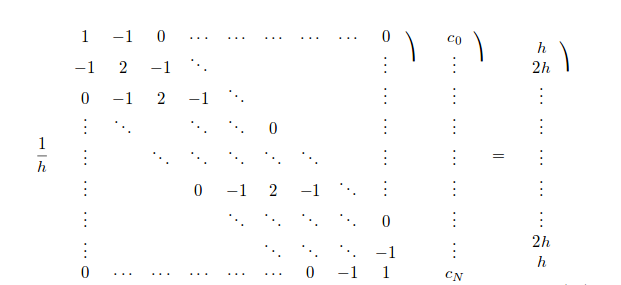
\includegraphics[scale=0.4]{unmod.png}
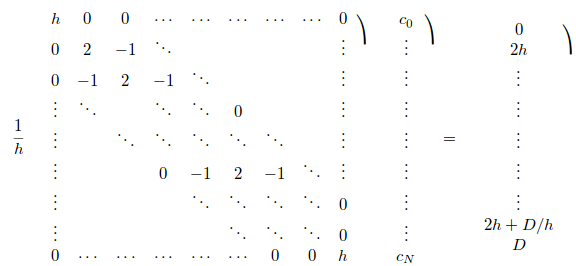
\includegraphics[scale=0.4]{mod.png}
\end{figure}
It can be shown that this matrix is  Symmetric Positive Definite, and hence CG is a good choice. Further what preconditioner
\begin{itemize}
\item Incomplete LU factorization ILU (Gaussians) is a robust-allaround preconditioner
\item AMG Algebraic multigrid, made for a matrix with positive and dominant diagonal entries. \newline
source(Parallel Algebraic Multigrid for the Pressure Poisson Equation in a Finite Element Navier-Stokes Solver)
\item The Jacobi preconditioner is one of the simplest forms of preconditioning, in which the preconditioner is chosen to be the diagonal of the matrix \newline
$P = diag(A)$, and by assuming $A_{ii} \neq 0$ we get $P_{ij}^-1 = \frac{\delta_{ij}}{A{ij}}$
\end{itemize}

\newpage

\begin{figure}
\centering
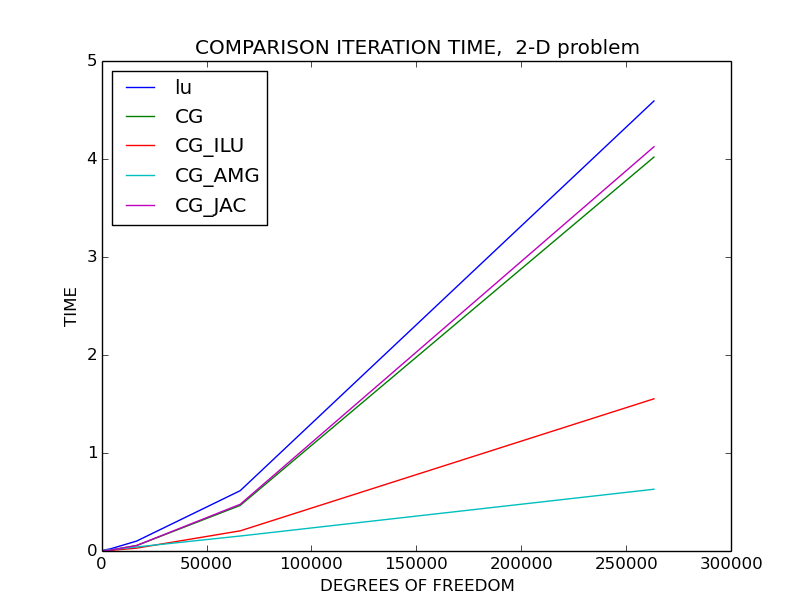
\includegraphics[scale=0.4]{comparefig.png}
\end{figure}

\begin{table}[h!]
\caption {Computationtime} 
\centering
\begin{tabular}{|c|c|c|c|c|c|c|c}
\hline
\rowcolor{LightCyan}
 N      &         32 &         64 &       128 &      256 &      512 \\
\hline
 lu     & 0.00644588 & 0.018074   & 0.112046  & 0.635943 & 4.71949  \\
 \rowcolor{LightCyan}
 cg     & 0.00135112 & 0.00682712 & 0.0620949 & 0.506644 & 4.14403  \\
 cg\_ilu & 0.00110793 & 0.00405598 & 0.029743  & 0.204767 & 1.5899   \\
 \rowcolor{LightCyan}
 cg\_amg & 0.00557399 & 0.0104449  & 0.0394349 & 0.149639 & 0.655219 \\
 cg\_jac & 0.001091   & 0.00739598 & 0.05532   & 0.499357 & 4.55105  \\
\hline
\end{tabular}
\end{table}

\begin{table}[h!]
\caption {Computationtime} 
\centering
\begin{tabular}{|c|c|c|c|c|c|c|c}
\hline
\rowcolor{LightCyan}
 N      &   32 &   64 &   128 &   256 &   512 \\ 
\hline
 lu     &    1 &    1 &     1 &     1 &     1 \\ 
 \rowcolor{LightCyan} \hline
 cg     &   50 &  100 &   203 &   409 &   827 \\ 
 cg\_ilu &   16 &   26 &    50 &    98 &   189 \\ 
 \rowcolor{LightCyan} 
 cg\_amg &    4 &    4 &     4 &     3 &     3 \\ 
 cg\_jac &   50 &  100 &   203 &   409 &   827 \\

\hline
\end{tabular}
\end{table}

\newpage \newpage
\section*{TASK 6: Linear Elasticity}
\textbf{Describe a variational formulation of the linear elasticity equation.  Dis-
cuss appropriate boundary conditions, problems associated with rigid mo-
tions and Korn's lemma.  Discuss the locking phenomena and mixed formu-
lations that avoid locking.}

\subsection*{Describe a variational formulation of the linear elasticity equation.}
Origin of equation. Define stress tensor $\sigma$. 
\begin{align*}
\nabla \cdot \sigma = f \hspace{2mm} \text{Newtons 2.law }
\end{align*}
Introducing Hookes law for linear elastic substance
\begin{align*}
\sigma = \lambda tr(\epsilon(u)) \delta + 2 \mu \epsilon(u); \hspace{3mm} \epsilon(u) = \frac{1}{2}(\nabla u + \nabla u^T) \\ 
\sigma_{ij} = \lambda \nabla \dot u \delta{ij} + 2 \mu \epsilon{ij}
\end{align*} 
Where $\mu, \lambda$ Lame's constants. Insertion in newtons 2.law yields
\begin{align*}
&\nabla \cdot \sigma = 2 \nabla \cdot \mu \epsilon(u) + \lambda \nabla \cdot tr(\epsilon(u)) \\
&- \mu \Delta u - \lambda \nabla \nabla \cdot u = f
\end{align*}

Solving using finite element method, is divided into 4 steps \newline
\textbf{1. Set up the strong form of the PDE} 
\begin{align*}
- \mu \Delta u - \lambda \nabla \nabla \cdot u = f \hspace{2mm} \text{in} \hspace{1mm} \Omega  \\
u = u_e \hspace{2mm} \text{in} \hspace{1mm} \partial \Omega
\end{align*} 
\textbf{2. Obtain the weak form of the PDE} multiply the equation with a test function v and integrate by parts
\begin{align*}
\mu \int \Delta u v \hspace{1mm} dx + \lambda \int \nabla \nabla \cdot u v \hspace{1mm} dx = \int f v dx\\ 
\mu \langle \nabla u \,, \nabla v \rangle + \lambda \langle \nabla \nabla \cdot u \,, v \rangle 
= \langle f \,, v \rangle
\end{align*}

\textbf{3. Finite Element method} We discretize the problem trying to find a solution in a descrete trial space and descrete test function.

We now define our problem as, find $u_h \in V_h \subset V$ such that
\begin{align*}
\mu \int \Delta u_h v_h \hspace{1mm} dx + \lambda \int \nabla \nabla \cdot u_h v_h \hspace{1mm} dx = \int f v_h dx \hspace{2mm} \forall v_h \in V_h \\ 
\mu \langle \nabla u_h \,, \nabla v_h \rangle + \lambda \langle \nabla \nabla \cdot u_h \,, v_h \rangle = \langle f \,, v_h \rangle
\end{align*}
\textbf{4. Solution algorithm} Solve linear system.....

\subsection*{Discuss appropriate boundary conditions, problems associated with rigid motions and Korn's lemma.}  
For linear elasticity appropriate boundary conditions must either be \textit{Plane Displacements} $u(x) = x - X(x)$ 
or \textit{Plane Tractions} $\tau = \sigma \cdot \textbf{n}$ or $\sigma \cdot \textbf{n} ds$ on the whole boundary. 
Example fluid Pressure, pressure along a boundary $\Omega$, then $\tau = -p\cdot \textbf{n}$
\begin{align*}
\nabla \nabla \cdot = \nabla^2 + \nabla \times (\nabla \times) \\
\text{Any field in} L_2 \hspace{2mm} v = \nabla \theta + \nabla \times \psi \\
\text{From identities} \hspace{2mm} \nabla \times (\nabla \psi) = 0 \hspace{2mm} \text{and} \hspace{1mm} \nabla \cdot ( \nabla \times F) = 0
\end{align*}
\textbf{Rigid motion} defined as 
\begin{align*}
\text{In 2D} \hspace{2mm} v = c + b 
   \begin{bmatrix}
         y \\
         -x
        \end{bmatrix}
        \hspace{2mm} c \in R^2 \hspace{1mm} \text{and} \hspace{1mm} b \in R
\end{align*}
\textbf{Problem with rigid motion} Our system $= 0$ \newline
\textbf{Korn's Lemma} \newline
Garanties a unique solution for the case of Dirichlet conditions on the boundary. Korns 1. inequality states
\begin{align*}
||\epsilon(u)||_{L_2} \geq C ||u||_{L_2} \hspace{2mm} \forall u \in H_0^1 
\end{align*}

\subsection*{ Discuss the locking phenomena and mixed formulations that avoid locking.}
\textbf{Locking} is a numerical artifact occuring when $\lambda >> \mu$, meaning the solid reaches and incompressible state. Here the displacements gets
very small. \newline
\textbf{The Problem?} The elements we are using in this course doesn't represent divergence fairly well, as $\nabla \nabla \cdot u$ gets bigger, the bad 
representation pollutes the numerical results. \newline
\textbf{WORKAROUND} \newline
Attack the divergence term by introducing mixed function space, to get a simulated stokes problem such that
\begin{align*}
p = \lambda \nabla \cdot u \\
- \u \Delta^2 u - \nabla p = f \\ 
\nabla \cdot u = \frac{p}{\lambda}
\end{align*}



\end{document}
